\documentclass[12pt, a4paper]{article}

\usepackage{makra}

\author{Maksymilian~Kicki}
\title{Mała przygoda~w~wielkim świecie matematyki}
\date{}

\linespread{1.1}
\hyphenation{naturalną potęgą liczby}
\begin{document}
\maketitle

\tableofcontents
\newpage
\section{Małe wprowadzenie}
\label{sec:Male_wprowadzenie}
\textbf{Matematyka} to królowa nauk. Wszyscy się z tym zgodzą (a w zaszadzie powinni). Natomiast niekażdy zgodzi się, że jest ona prosta. Wielu ludzi twierdzi, że matematyka dla nich to ,,\textbf{czarna magia}''. Matematyka pozwala nam w jakiś sposób opisać zjawiska, które nas otaczają, uogólnić przypadki, z którymi często się spotykamy. W dzisiejszych czasach bez znajomości podstaw matematycznych ludzie nie mogliby normalne egzystować. Skąd niby mieliby wiedzieć ile dostaną wypłaty? Jak doszliby do tego ile reszty musi im wydać pani w sklepie? Albo też ile metrów siatki trzeba kupić żeby ogrodzić swoją posiadłość? Są to przyziemne przypadki, jednak jakże istotne w naszym codziennym życiu. Nie wspominając już o tym, że bez skomplikowanych działań i obliczeń matematycznych nie zostałaby stworzona żadna maszyna. Nie powstałyby pociągi, samochody, lodówki i oczywiście nie byłoby komputerów. Chociaż dzięki tym ostatnim liczenie zostało nam bardzo ułatwione, to każdy powinien mieć jakiekolwiek pojęcie o podstawowych działaniach matematycznych. Niektórzy zainteresują się tematem mniej, a inni bardziej (jak ja). Dlatego też postanowiłem stworzyć małe wprowadzenie do wielkiego i ciekawego świata matematyki.
\begin{figure}[htbp]
	\centering
		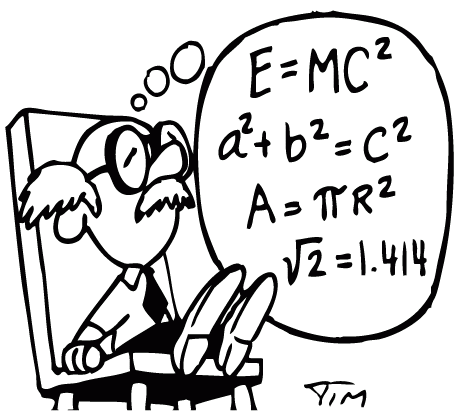
\includegraphics[width=0.50\textwidth]{matematyka.png}
	\label{fig:matematyka}
\end{figure}

\newpage
\section{Ułamki zwykłe i dziesiętne oraz procenty}
\label{subsec:Ulamki}
Zacznijmy od czegoś prostego. Zakładając, że dodawanie, odejmowanie, mnożenie i dzielenie liczb naturalnych nie powinno sprawiać problemów, weźmiemy pod lupę \textbf{ułamki}.
\subsection{Definicje}
\begin{itemize}
\item \underline{Ułamek} - wyrażenie lub liczba postaci $\frac{a}{b}$ (czasami zapisujemy $a/b$, rzadziej $a:b$), gdzie \emph{a} nazywamy \textbf{licznikiem} ułamka, a \emph{b} nazywamy \textbf{mianownikiem} ułamka. Kreskę poziomą między licznikiem i mianownikiem nazywamy \textbf{kreską ułamkową}. Ułamek zapisany przy pomocy licznika, mianownika i kreski ułamkowej nazywamy \textbf{ułamkiem zwykłym} np.
		\begin{itemize}
			\item [*]$\frac{7}{8}$
			\item [*]$\frac{49}{99}$
			\item [*]$\frac{17}{12}$. 
		\end{itemize}
\item \underline{Ułamek dziesiętny} - ułamek, w którym mianownik jest \textbf{naturalną potęgą liczby} 10, np. 
		\begin{itemize}
			\item [*]$\frac{7}{10}$
			\item [*]$\frac{49}{100}$
			\item [*]$\frac{17}{10^4}$. 
		\end{itemize}
	Ułamek dziesiętny zapisujemy najczęściej używając \textbf{przecinka}, a nie kreski ułamkowej, np. 
		\begin{itemize}
			\item [*]$\frac{7}{10} = 0,7$
			\item [*]$\frac{49}{100} = 0,49$
			\item [*]$\frac{17}{10^4} = 0,0017$.
	\end{itemize}
\end{itemize}\cite{matemaks} 
\newpage\subsection{Ułamek zwykły}
Każdy ułamek zwykły składa się z trzech elementów – licznika, mianownika i kreski ułamkowej. Kreska ułamkowa symbolizuje znak dzielenia.
\begin{figure}[htbp]
	\centering
		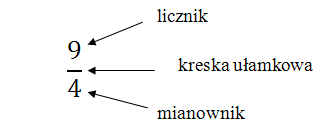
\includegraphics[width=0.40\textwidth]{definicja.png}
	\label{fig:definicja}
\end{figure}
\newline Dzięki ułamkom możemy zapisywać liczby, które nie są całkowite.
\underline{Przykład:}
\begin{figure}[htbp]
	\centering
		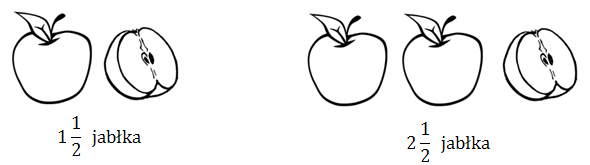
\includegraphics[width=0.55\textwidth]{jablka1.png}
	\label{fig:jablka1}
\end{figure}\cite{matemaks} 
\subsection{Działania na ułamkach}
\begin{itemize}
	\item Rozszerzanie i skracanie ułamków: ułamek \textbf{rozszerzamy} mnożąc, a \textbf{skracamy} dzieląc jego licznik i mianownik przez liczbę różną od \texttt{zera}.
	\newline\underline{Przykłady:} 
	\begin{itemize}
	\item[*]$\frac{1}{2}=\frac{1\cdot5}{2\cdot5}=\frac{5}{10}$
	\item[*]$\frac{10}{15}=\frac{10\div5}{15\div5}=\frac{2}{3}$
	\end{itemize}
	\item Dodawanie~i odejmowanie ułamków: aby dodać lub odjąć ułamki zwykłe, to należy je wcześniej sprowadzić do \textbf{wspólnego mianownika}.
	\newline\underline{Przykłady:} 
		\begin{itemize}
	\item[*]$\frac{2}{3}+\frac{3}{4}=\frac{2\cdot4}{3\cdot4}+\frac{3\cdot3}{4\cdot3}=\frac{8}{12}+\frac{9}{12}=\frac{17}{12}=1\frac{5}{12}$
	\item[*]$\frac{1}{3}-\frac{2}{7}=\frac{1\cdot7}{3\cdot7}-\frac{2\cdot3}{7\cdot3}=\frac{7}{21}-\frac{6}{21}=\frac{1}{21}$
		\end{itemize}
	\item Mnożenie ułamków: po prostu, licznik razy licznik i mianownik razy mianownik.
	\newline\underline{Przykład:} 
		\begin{itemize}
		\item[*]$\frac{2}{3}\cdot\frac{3}{5}=\frac{2\cdot3}{3\cdot5}=\frac{6}{15}=\frac{2}{5}$
		\end{itemize}
	\newpage
	\item Dzielenie ułamków: kiedy musimy podzielić jeden ułamek przez drugi, to \textbf{zamieniamy} dzielenie na mnożenie. Mnożymy wówczas pierwszy ułamek przez \textbf{odwrotność} drugiego ułamka.
	\newline\underline{Przykład:} 
		\begin{itemize}
		\item[*]$\frac{2}{3}\div\frac{3}{5}=\frac{2}{3}\cdot\frac{5}{3}=\frac{2\cdot5}{3\cdot3}=\frac{10}{9}=1\frac{1}{9}$
		\end{itemize}
\end{itemize}\cite{matemaks} 

\subsection{Procenty - co to jest?} 
\label{subsubsec:Procenty}
Słowo procent pochodzi od łacińskiego wyrażenia \emph{per centum} - "na sto".
Jeden procent zapisujemy symbolem $1\%$. Oznacza on jedną setną część całości.
Jeżeli mówimy, że $23\%$ Polaków ma oczy niebieskie, to znaczy, że przeciętnie na 100 Polaków jest 23 takich, którzy mają oczy niebieskie. Można też powiedzieć, że $\frac{23}{100}$ wszystkich Polaków ma oczy niebieskie.\newline
Możemy zatem wyrażać procenty w postaci ułamków:
\begin{itemize}
	\item \textbf{zwykłych} - $1\%=\frac{1}{100}$
	\item \textbf{dziesiętnych} - $1\%=0,01$
\end{itemize}
\underline{Przykłady:}
\begin{enumerate}
		\item $7\%=\frac{7}{100}=0,07$
		\item $16\%=\frac{16}{100}=0,16$
		\item $49\%=\frac{49}{100}=0,49$
		\item $71\%=\frac{71}{100}=0,71$
		\item $175\%=\frac{175}{100}=1,75$
	\end{enumerate}\cite{matemaks} 
\newpage
\section{Wielka, lecz krótka podróż}
\label{sec:Wielka}
Po przyjemnych rozgrzewkach na poziomie szkoły podstawowej~i gimnazjalnej przejdźmy do czegoś trudniejszego. Rozpoczniemy krótką podróż po tajnikach matematyki. W~tym rozdziale zajmiemy się krótkim omówieniem \textbf{układadów równań} i \textbf{macierzy}. Dodatkowo wspomnimy również~o kilku innych ciekawych rzeczach.
\subsection{Układy równań}
\label{rownania}
Wyrażenie postaci $x+3y=6$ nazywamy równaniem liniowym~z dwiema niewiadomymi. Dwa lub więcej takich równań (jak~i równań kwadratowych) połączonych klamrą nazywamy \textbf{układem równań}.
\newline\underline{Przykład} \eqref{eq:nr1}, \eqref{eq:nr2} i \eqref{eq:nr3}:
\begin{equation}
\label{eq:nr1}
	\left \{	
	\begin{array}{ll}
	x + 3y = 7 \\
	2x - y = 4 \\
		\end{array}
		\right.
\end{equation}
\begin{equation}
\label{eq:nr2}
	\left \{	
	\begin{array}{ll}
	x^2 + 3y = 49 \\
	4x - y^2 = 75 \\
		\end{array}
		\right.
	\end{equation}
	\begin{equation}
\label{eq:nr3}
	\left \{	
	\begin{array}{ll}
	x_1 - 3x_2 + 2x_3 - x_4 = 49 \\
	-2x_1 - x_2 + 5x_3 + 2x_4 = 15 \\
	2x_1 + x_2 + x_3 - 3x_4 = 13 \\
	x_1 - 2x_2 + 2x_3 + 9x_4 = 34\\
		\end{array}
		\right.
	\end{equation}\cite{matemaks} 
\subsection{Macierze}
\label{sec:Macierze}
Pojęcie \textbf{macierzy} wprowadzono, aby uprościć rozwiązywanie układów równań liniowych. Rozwiązanie dużych układów równań wiązało się z wykonywaniem wielu żmudnych działań, co groziło łatwą pomyłką. Nie jest ciężko rozwiązać układ z 2 niewiadomymi i z 2 równaniami, ale gdybyśmy musieli rozwiązywać układy 4 równań z 4 niewiadomymi, lub jeszcze większe mielibyśmy nie mały kłopot. Do rozwiązywania tego typu problemów przydają się właśnie macierze. Rozmiar układu nie ma większego znaczenia, gdy rozwiązujemy go za pomocą macierzy.
\newline Ogólna postać macierzy jest następująca:
\begin{displaymath}
\mathbf{X} =
\left[ \begin{array}{cccc}
x_{11} & x_{12} & \ldots & x_{1n}\\
x_{21} & x_{22} & \ldots & x_{2n}\\
\vdots & \vdots & \ddots & \vdots\\
x_{n1} & x_{n2} & \ldots & x_{nn}
\end{array} \right]
\end{displaymath}
 W każdej macierzy możemy wyróżnić \textbf{kolumny} oraz \textbf{wiersze}.
\begin{figure}[htbp]
	\centering
		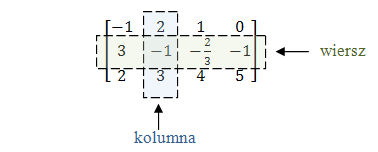
\includegraphics[width=0.60\textwidth]{macierz3.png}
	\label{fig:macierz3}
\end{figure}
\newline Aby rozwiązać układ za pomocą macierzy wypisujemy w macierzy kolejno wszystkie \textbf{współczynniki liczbowe} z naszego równania, np:
\begin{figure}[htbp]
	\centering
		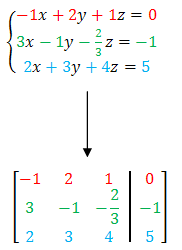
\includegraphics[width=0.30\textwidth]{macierz2.png}
	\label{fig:macierz2}
\end{figure}
\newline\textbf{Pionowa kreska}, w powyższej macierzy, oddziela współczynniki wolne, stojące po prawej stronie znaków równości. Nie ma konieczności pisania tej kreski. Stosuje się ją tylko w celu uzyskania lepszej przejrzystości.
\newpage Na macierzach (podobnie jak na układach równań) można wykonywać trzy proste operacje:
\begin{itemize}
\item dodać do jednego wiersza macierzy inny wiersz pomnożony przez liczbę,
\item zamienić dwa wiersze miejscami,
\item pomnożyć wiersz przez liczbę różną od zera.
\end{itemize}
I to właśnie za pomocą tych operacji rozwiązywane są macierze (a za pomocą macierzy układy równań).\cite{matemaks} 
\newline\begin{center}\Huge Magia!\end{center}
\begin{figure}[hp]
	\centering
		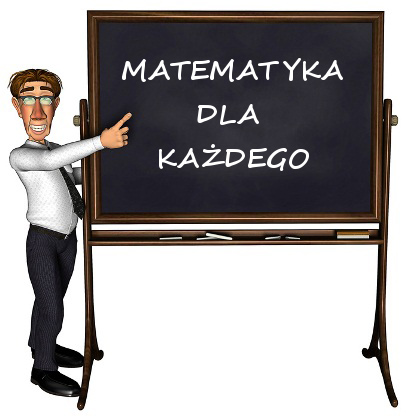
\includegraphics[width=0.65\textwidth]{matematyk.jpg}
	\label{fig:matematyk}
\end{figure}

\normalsize
\newpage
\subsection{Logika matematyczna}
Bardziej w ramach ciekawostki niż objaśnienia, wspomnę jeszcze o logice matematycznej. Czy wiedziałeś, że z punktu widzenia matematyki zdanie:
\begin{quote}
\emph{Jeżeli Jan zna logikę, to jeśli Jan nie zna logiki to $2 + 2 = 15$} 
\end{quote}
jest zawsze prawdzie i jest tak zwaną tautologią\footnote{Tautologia – wyrażenie, które jest prawdziwe na mocy swojej formy – budowy}? 
\newline Dlaczego? Otóż przyjmijmy następujące oznaczenia
\begin{itemize}
\item \~ - ,,Nieprawda, że($\ldots$)''
\item $\Rightarrow$ - ,,Jeżeli($\ldots$)z tego wynika, że($\ldots$)''
\item p - Jan zna logikę
\item $\neg$p - Jan nie zna logiki
\item q - $2 + 2 = 15$
\end{itemize}
Wtedy mamy:
\begin{quote}
p $\Rightarrow$ ($\neg$p $\Rightarrow$ r)
\end{quote}
Kożystając z tabeli wartościowania zdań\footnote{1 - oznacza zdanie prawdziwe, 0 - zdanie nieprawdziwe} :
\begin{center}
\begin{tabular}{|c|c|c|c|c|}
\hline
p & q & $\neg$p & $\neg$p $\Rightarrow$ q & p $\Rightarrow$ ($\neg$p $\Rightarrow$ q)\\\hline
0 & 0 & 1 & 0 & 1\\\hline
0 & 1 & 1 & 1 & 1\\\hline
1 & 0 & 0 & 1 & 1\\\hline
1 & 1 & 0 & 1 & 1\\\hline
\end{tabular}
\end{center}
udowodniliśmy, że zdanie te jest zawsze prawdziwe.\cite{wstep}
\newpage
\section{Przerwa? No jasne}
Wszyscy wiedzą, że gdyby nie przerwy w pracy i nauce to wszystko byłoby cięższe. Także, jeśli przeczytałeś/łaś \emph{to} za jednym podejściem to należy Ci się zasłużona przerwa. Zobacz jeszcze jak wspaniałe są obrazki opisane za pomocą wzorów matematycznych, a nie pixeli (grafika wektorowa). Miłej zabawy i do zobaczenia!
\begin{figure}[htbp]
	\centering
		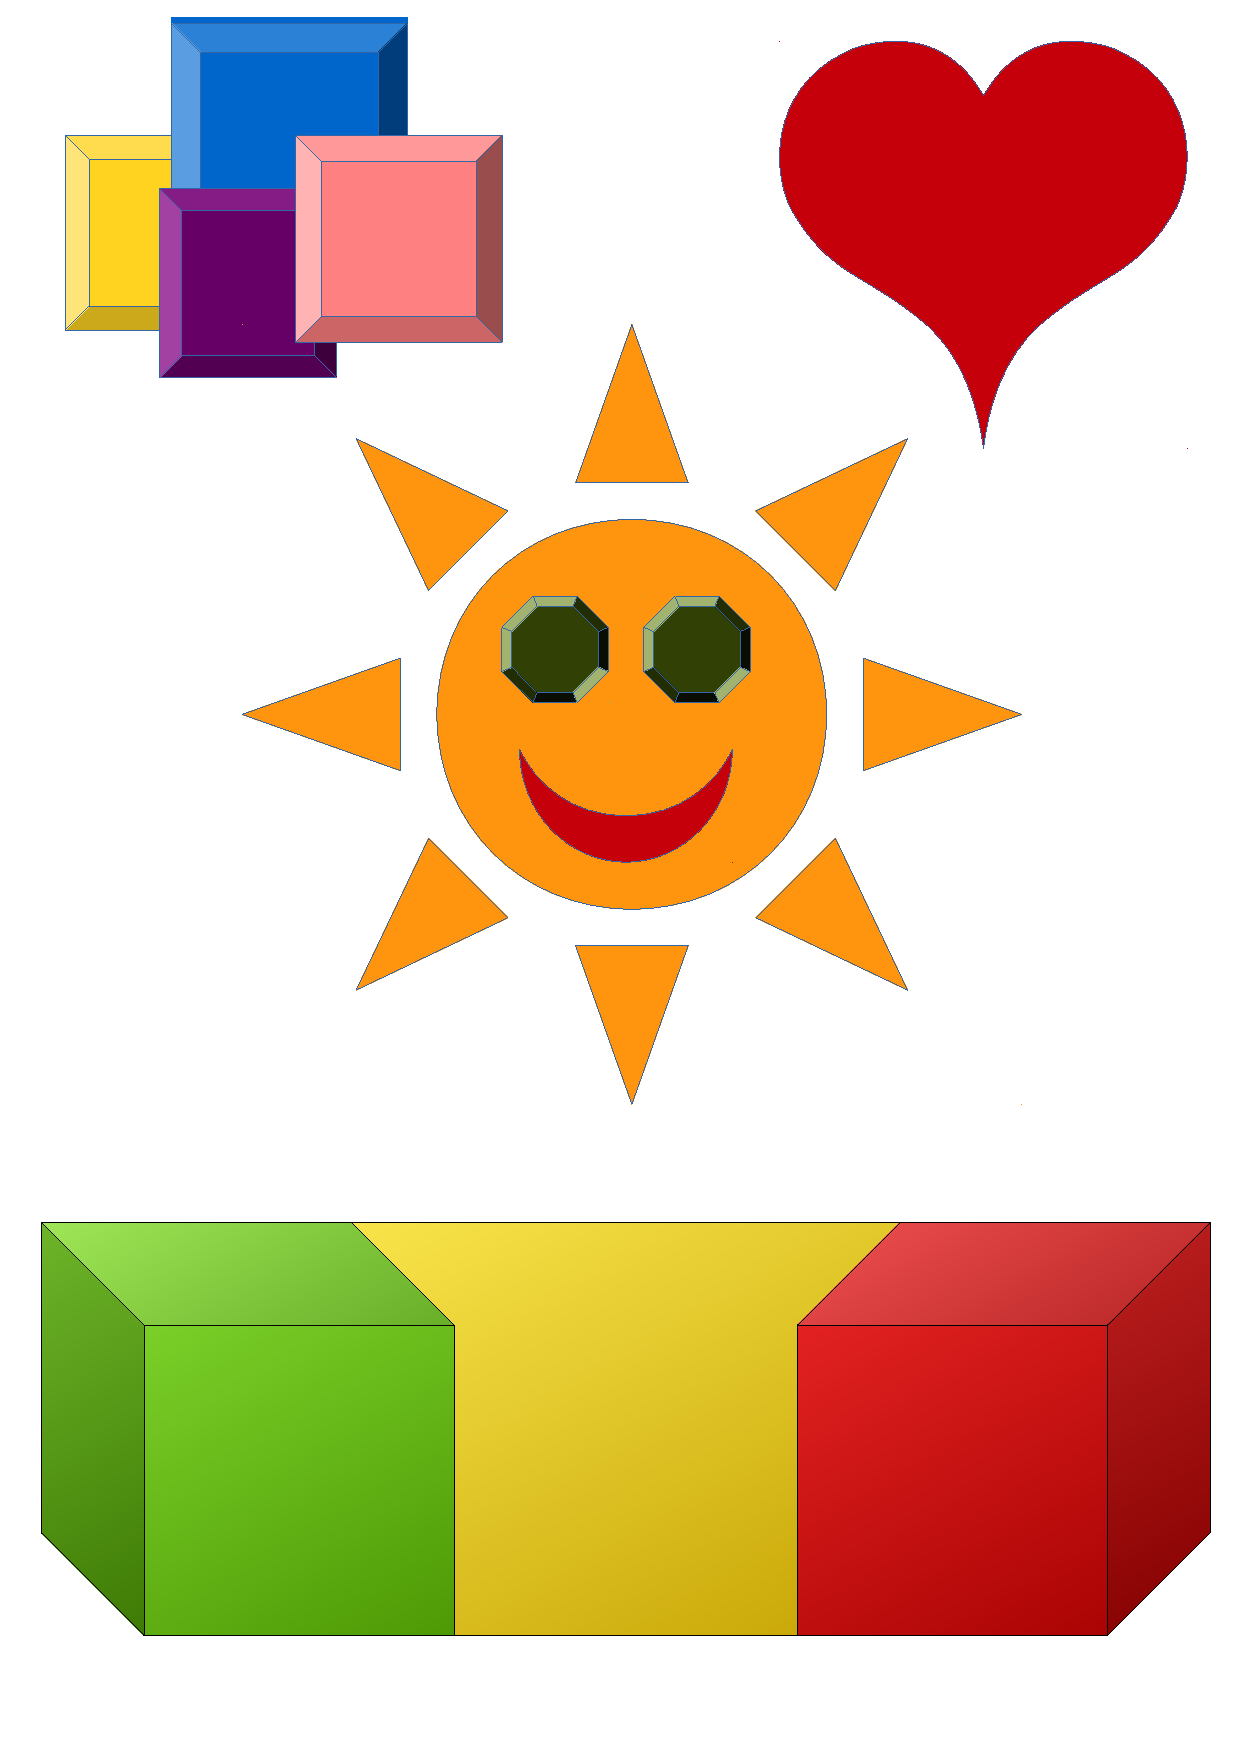
\includegraphics[width=0.50\textwidth]{lol2.pdf}
	\label{fig:lol2}
\end{figure}



\bibliographystyle{plain}
\bibliography{mojaBib}
 
\end{document}
